\documentclass[../main]{subfiles}
\begin{document}
% \setcounter{section}{0}
\section{線形代数}
%------------------------------------------------------------
\begin{figure}[H]
    \centering
\begin{tikzpicture}
    \draw (0,0) -- (3.5,0) node[right]{$x$};
    \draw (0,0) -- (0,3.5) node[above]{$y$};
    \draw[very thick] (1,2) -- (3,3);
    \draw[very thick] (2,1) -- (3,3);
    \fill[color=gray!20] (0,0) -- (1,2) -- (3,3) -- (2,1) -- cycle;
    \draw[-latex,very thick,graphcolor] (0,0) -- (1,2) node[above]{$\vec{b}$};
    \draw[-latex,very thick,graphcolor] (0,0) -- (2,1) node[right]{$\vec{a}$};
\end{tikzpicture}
\end{figure}
%------------------------------------------------------------
\begin{figure}[H]
    \centering
\begin{tikzpicture}
    \draw (0,0) -- (3.5,0);
    \draw (0,0) -- (0,3.5);
    \draw[very thick] (1,2) -- (3,3);
    \draw[very thick] (2,1) -- (3,3);
    \fill[color=gray!20] (0,0) -- (1,2) -- (3,3) -- (2,1) -- cycle;
    \draw[dotted] (1,0) node[below]{$b_x$} -- (1,2);
    \draw[dotted,very thin] (2,0) node[below]{$a_x$} -- (2,1);
    \draw[dotted,very thin] (0,1) node[left]{$a_y$} -- (2,1);
    \draw[dotted,very thin] (0,2) node[left]{$b_y$} -- (1,2);
    \draw[-latex,very thick,graphcolor] (0,0) -- (1,2) node[above]{$\vec{b}$};
    \draw[-latex,very thick,graphcolor] (0,0) -- (2,1) node[right]{$\vec{a}$};
    \path (0,0) coordinate (O);
    \path (1,2) coordinate (A);
    \path (2,1) coordinate (B);
    \path (2,0) coordinate (X);
    \tkzMarkAngle[size=0.9](X,O,A)
    \tkzLabelAngle[pos=1.0,yshift=2.0](X,O,A){\scriptsize$\beta$}
    \tkzMarkAngle[size=0.5](X,O,B)
    \tkzLabelAngle[pos=0.7](X,O,B){\scriptsize$\alpha$}
\end{tikzpicture}
\end{figure}
%------------------------------------------------------------
\begin{figure}[H]
    \centering
\begin{tikzpicture}
    \draw[->] (-1,0) -- (5,0) node(xaxis)[right] {$x$};
    \draw[->] (0,-1) -- (0,4) node(yaxis)[above] {$y$};
    \fill[graphcolor] (2,3) circle (1.5pt);
    \fill[graphcolor] (4,1) circle (1.5pt);
    \draw[-latex,very thick,graphcolor] (0,0) -- (2,3) node[above]{$\vec{a} (2,3)$};
    \draw[-latex,very thick,graphcolor] (0,0) -- (4,1) node[above]{$\vec{b} (4,1)$};
    \path (0,0) coordinate (O) node[below right] {$O$};
\end{tikzpicture}
\end{figure}
%------------------------------------------------------------
\begin{figure}[H]
    \centering
\begin{tikzpicture}
    \draw[->] (-1,0) -- (5,0) node(xaxis)[right] {$x$};
    \draw[->] (0,-1) -- (0,4) node(yaxis)[above] {$y$};
    \draw[-latex,very thick,graphcolor] (2,1) -- node[left]{$\vec{a}$} (4,4);
    \draw[-latex,very thick,graphcolor] (0,0) -- node[left]{$\vec{a}$} (2,3);
    \draw[-latex,very thick,graphcolor] (0,0) -- node[below]{$\vec{b}$} (4,1);
    \draw[-latex,very thick,graphcolor] (0,-1) -- node[below]{$\vec{b}$} (4,0);
    \path (0,0) coordinate (O) node[below right] {$O$};
\end{tikzpicture}
\end{figure}
%------------------------------------------------------------
\begin{figure}[H]
    \centering
\begin{minipage}{.45\textwidth}
    \begin{tikzpicture}
        \draw[->] (0,0) -- (3,0) node(xaxis)[right] {$x$};
        \draw[->] (0,0) -- (0,3) node(yaxis)[above] {$y$};
        \draw[dashed,very thin] (0,2) node[left]{$a_y$} -- (2,2);
        \draw[dashed,very thin] (2,0) node[below]{$a_x$} -- (2,2);
        \fill[graphcolor] (2,2) circle (1.5pt);
        \draw[-latex,very thick,graphcolor] (0,0) -- (2,2) node[above]{$\vec{a}$} ;
    \end{tikzpicture}
\end{minipage}
\begin{minipage}{.45\textwidth}
    \begin{tikzpicture}
        \draw[->] (0,0) -- (3,0) node(xaxis)[right] {$x$};
        \draw[->] (0,0) -- (0,3) node(yaxis)[above] {$y$};
        \fill[graphcolor] (2,2) circle (1.5pt);
        \draw[-latex,very thick,graphcolor] (0,0) -- node[left]{$r$} (2,2) node[above right]{$\vec{a}=(r,\theta)$};
        \path (0,0) coordinate (O);
        \path (3,0) coordinate (X);
        \path (2,2) coordinate (A);
        \tkzMarkAngle[size=0.5](X,O,A);
        \tkzLabelAngle[pos=0.7](X,O,A){$\theta$};
    \end{tikzpicture}
\end{minipage}
\end{figure}
%------------------------------------------------------------
\begin{figure}[H]
    \centering
\begin{tikzpicture}
    \draw (0,0) -- (3.5,0);
    \draw (0,0) -- (0,3.5);
    \draw[dashed,very thin] (1.5,0) node[below]{$a_x$} -- (1.5,3);
    \draw[dashed,very thin] (3,0) node[below]{$b_x$} -- (3,1.5);
    \draw[dashed,very thin] (0,1.5) node[left]{$a_y$} -- (3,1.5);
    \draw[dashed,very thin] (0,3) node[left]{$b_y$} -- (1.5,3);
    \draw[-latex,very thick,graphcolor] (0,0) -- (1.5,3) node[above]{$\vec{a}$};
    \draw[-latex,very thick,graphcolor] (0,0) -- (3,1.5) node[above]{$\vec{b}$};
    \path (0,0) coordinate (O);
    \path (1,2) coordinate (A);
    \path (2,1) coordinate (B);
    \tkzMarkAngle[size=0.5](B,O,A)
    \tkzLabelAngle[pos=0.7](B,O,A){$\theta$}
\end{tikzpicture}
\end{figure}
%------------------------------------------------------------
\begin{figure}[H]
    \centering
\begin{tikzpicture}
    \draw (0,0) -- (3.5,0);
    \draw (0,0) -- (0,3.5);
    \draw[dashed,very thin] (1.5,0) node[below]{$a_x$} -- (1.5,3);
    \draw[dashed,very thin] (3,0) node[below]{$b_x$} -- (3,1.5);
    \draw[dashed,very thin] (0,1.5) node[left]{$b_y$} -- (3,1.5);
    \draw[dashed,very thin] (0,3) node[left]{$a_y$} -- (1.5,3);
    \draw[-latex,very thick,graphcolor] (0,0) -- (1.5,3) node[above]{$\vec{a}$};
    \draw[-latex,very thick,graphcolor] (0,0) -- (3,1.5) node[above]{$\vec{b}$};
    \path (0,0) coordinate (O);
    \path (1,2) coordinate (A);
    \path (2,1) coordinate (B);
    \path (2,0) coordinate (X);
    \tkzMarkAngle[size=1.0](X,O,A)
    \tkzLabelAngle[pos=1.2](X,O,A){$\alpha$}
    \tkzMarkAngle[size=0.5](X,O,B)
    \tkzLabelAngle[pos=0.7](X,O,B){$\beta$}
\end{tikzpicture}
\end{figure}
%------------------------------------------------------------
\begin{figure}[H]
    \centering
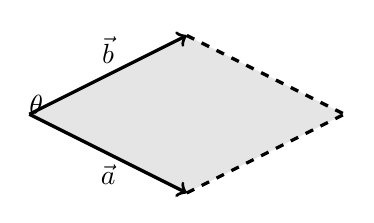
\begin{tikzpicture}
    \path (0,0) coordinate (P1);
    \path (2,-1) coordinate (P2);
    \path (4,0) coordinate (P3);
    \path (2,1) coordinate (P4);
    % \fill[pattern=north west lines,pattern color=graphcolor] (P1) -- (P2) -- (P3) -- (P4) -- cycle;
    \fill[color=gray!20] (P1) -- (P2) -- (P3) -- (P4) -- cycle;
    \draw[->,very thick] (0,0) -- node[below]{$\vec{a}$} (2,-1);
    \draw[->,very thick] (0,0) -- node[above]{$\vec{b}$} (2,1);
    \draw[very thick,dashed] (2,-1) -- (4,0);
    \draw[very thick,dashed] (2,1) -- (4,0);
    \tkzMarkAngle[size=0.5](P2,P1,P4)
    \tkzLabelAngle[pos=0.7](P2,P1,P4){$\theta$}
\end{tikzpicture}
\end{figure}
%------------------------------------------------------------
\begin{tikzpicture}
    \draw[->,very thick] (0,0) -- (3,.5) node[right]{$\vec{a}$};
    \draw[->,very thick] (0,0) -- (0,3) node[above]{$\vec{b}$};
    \path (0,0) coordinate (O) node[above right]{$\theta$};
    \path (.5,.5) coordinate (P1);
    \path (3.5,1) coordinate (P2);
    \path (3.5,4.0) coordinate (P3);
    \path (.5,3.5) coordinate (P4);
    \draw[fill,pattern=north west lines,pattern color=graphcolor] (P1) -- (P2) -- (P3) -- (P4) -- cycle;
    \path (1,4.5) node[right]{$|\vec{c}|=|\vec{a}||\vec{b}|\sin\theta$};
\end{tikzpicture}
%------------------------------------------------------------
\begin{figure}[H]
    \centering
\begin{tikzpicture}
    \draw[->,very thick] (0,0) -- (3,0) node[right]{$\vec{a}$};
    \draw[->,very thick] (0,0) -- (2,1) node[above]{$\vec{b}$};
    \draw[->,very thick,graphcolor] (0,0) -- (0,2) node[above]{$\vec{a}\times\vec{b}$};
    \draw[->,very thick,graphsubcolor] (0,0) -- (0,-2) node[below]{$\vec{b}\times\vec{a}$};
    \path (0,0) coordinate (O);
    \path (3,0) coordinate (X);
    \path (2,1) coordinate (Y);
    \path (0,3) coordinate (Z);
    \tkzMarkAngle[size=1.0](X,O,Y)
    \tkzLabelAngle[pos=1.2](X,O,Y){$\theta$}
    \tkzMarkRightAngle[size=0.3](X,O,Z);
    \tkzMarkRightAngle[size=0.3](Y,O,Z);
    \draw[-latex,bend right,distance=.2cm] (2.8,0.2) to (2.2,0.8);
\end{tikzpicture}
\end{figure}
%------------------------------------------------------------
\begin{figure}[H]
    \centering
\begin{tikzpicture}
    \path (0,0) coordinate (O);
    \draw[->] (-1,0) -- (2.5,0) node[right]{$x$};
    \draw[->] (0,-1) -- (0,2.5) node[above]{$y$};
    \path (3,1) coordinate (B);
    \path (1,2) coordinate (A);
    \draw[->,very thick,graphcolor] (0,0) -- ($(O)!.8!(A)$) node[left]{$\vec{a}$};
    \draw[->,very thick,graphcolor] (0,0) -- ($(O)!.6!(B)$) node[below]{$\vec{b}$};
\end{tikzpicture}
\end{figure}
%------------------------------------------------------------
\begin{figure}[H]
    \centering
\begin{tikzpicture}
    \path (0,0) coordinate (O);
    \draw (-3,-1) -- (3,1) coordinate (B);
    \draw (-1,-2) -- (1,2) coordinate (A);
    \draw[->,very thick,graphcolor] (0,0) -- ($(O)!.8!(A)$) node[left]{$\vec{a}$};
    \draw[->,very thick,graphcolor] (0,0) -- ($(O)!.6!(B)$) node[below]{$\vec{b}$};
    \path (2.5,1.2) node[left]{$m\vec{a}+n\vec{b}$};
    \path (-1,1.2) node[left]{$m\vec{a}-n\vec{b}$};
    \path (-1,-1) node[left]{$-m\vec{a}-n\vec{b}$};
    \path (2.5,-1) node[left]{$-m\vec{a}+n\vec{b}$};
\end{tikzpicture}
\end{figure}
%------------------------------------------------------------
\begin{figure}[H]
    \centering
\begin{tikzpicture}
    \path (0,0) coordinate (O);
    \draw (O) -- (3,0) node[right]{$y$} coordinate (Y);
    \draw (O) -- (-1.5,-1.5) node[below]{$x$} coordinate (X);
    \draw (O) -- (0,3) node[above]{$z$} coordinate (Z);
    \draw[->,very thick,graphcolor] (0,0) -- ($(O)!.5!(X)$) node[below right]{$\vec{e}_x$};
    \draw[->,very thick,graphcolor] (0,0) -- ($(O)!.5!(Y)$) node[below]{$\vec{e}_y$};
    \draw[->,very thick,graphcolor] (0,0) -- ($(O)!.5!(Z)$) node[right]{$\vec{e}_z$};
    \path ($(O)!.5!(X)$) node[left]{1};
    \path ($(O)!.5!(Y)$) node[above]{1};
    \path ($(O)!.5!(Z)$) node[left]{1};
\end{tikzpicture}
\end{figure}
%------------------------------------------------------------
\begin{figure}[H]
    \centering
\begin{tikzpicture}
    \path (0,0) coordinate (O);
    \path (2,3) coordinate (A);
    \draw[very thick] (-3,2) -- (3,-2);
    \draw[->,very thick,graphcolor] (0,0) -- ($(O)!0.8!(A)$) node[above right]{$\vec{a}$};
    \draw[->] (O) -- (0,2) node[above]{$\vec{b}$};
    \draw[->] (O) -- (2,0);
    \draw[->] (O) -- (30:2) node[right]{$\vec{b}$};
    \draw[->] (O) -- (120:2);
    \draw[->] (O) -- (180:2) node[left]{$\vec{b}$};
    \draw[->] (O) -- (240:2);
    \draw[->] (O) -- (280:2);
    \path (340:2) node[right]{$\vec{a}\cdot\vec{b} > 0$};
    \path (300:2) node[right]{$\vec{a}\cdot\vec{b} < 0$};
\end{tikzpicture}
\end{figure}
%------------------------------------------------------------
\begin{figure}[H]
    \centering
\begin{tikzpicture}
    \path (0,0) coordinate (O);
    \path (3,2) coordinate (A);
    \draw (O) -- (4,0) coordinate (X);
    \draw (3,0) -- (3,2);
    \draw[->,very thick,graphcolor] (0,0) -- node[above]{$\vec{a}$} (3,2);
    \draw[->,very thick,graphcolor] (0,0) -- (1,0) node[below]{$\vec{e}$};
    \tkzMarkAngle[size=0.5](X,O,A)
    \tkzLabelAngle[pos=0.7](X,O,A){$\theta$}
\end{tikzpicture}
\end{figure}
%------------------------------------------------------------
%------------------------------------------------------------
%------------------------------------------------------------
%------------------------------------------------------------
%------------------------------------------------------------
\end{document}